\chapter{الأكسدة والاختزال في الكيمياء العضوية}\label{ch:b1:organic-redox}

قارورة نبيذ تُترك مفتوحة تتحول في غضون أيام إلى خل: إذ تستعمل البكتيريا
أكسجين الهواء لتؤكسد الإيثانول إلى حمض الإيثانويك. والكيتون
والكحول الذي يأتي منه يختلفان بذرتي هيدروجين --- وإذا عُدّ الأمر
كما ينبغي، بإلكترونين. ولا تشبه الأكسدة والاختزال في الكيمياء العضوية
تبادلات الإلكترونات بين أيونات الفلزات في \cref{ch:b1:nernst}،
لأن الإلكترونات تنتقل مع البروتونات أو مع أيونات الهيدريد، لكن
الحساب واحد. يعيّن هذا الفصل \omterm{def:b1:organic-redox:oxidation-level}{مستويات أكسدة} للكربون،
ويستعملها للتنبؤ بما يعطيه كل كحول عند أكسدته،
ويقدّم كواشف الهيدريد التي تختزل مركبات الكربونيل، مع
الانتباه إلى المجموعات التي يتركها كل كاشف دون مساس.

\begin{recall}
\omterm{def:b1:nernst:oxidation-number}{أعداد الأكسدة}، وأنصاف المعادلات وموازنة معادلات الأكسدة والاختزال موجودة
في \cref{ch:b1:nernst}؛ وأصناف الكحولات والكربونات في
\cref{ch:b1:electronic-effects}؛ \omterm{def:b1:acetals-protection:hemiacetal}{والأسيتالات} \omterm{def:b1:acetals-protection:protecting-group}{وحماية} مجموعات
الكربونيل في \cref{ch:b1:acetals-protection}؛ وإضافات غرينيار في
\cref{ch:b1:organomagnesium}.
\end{recall}

\begin{omfigure}
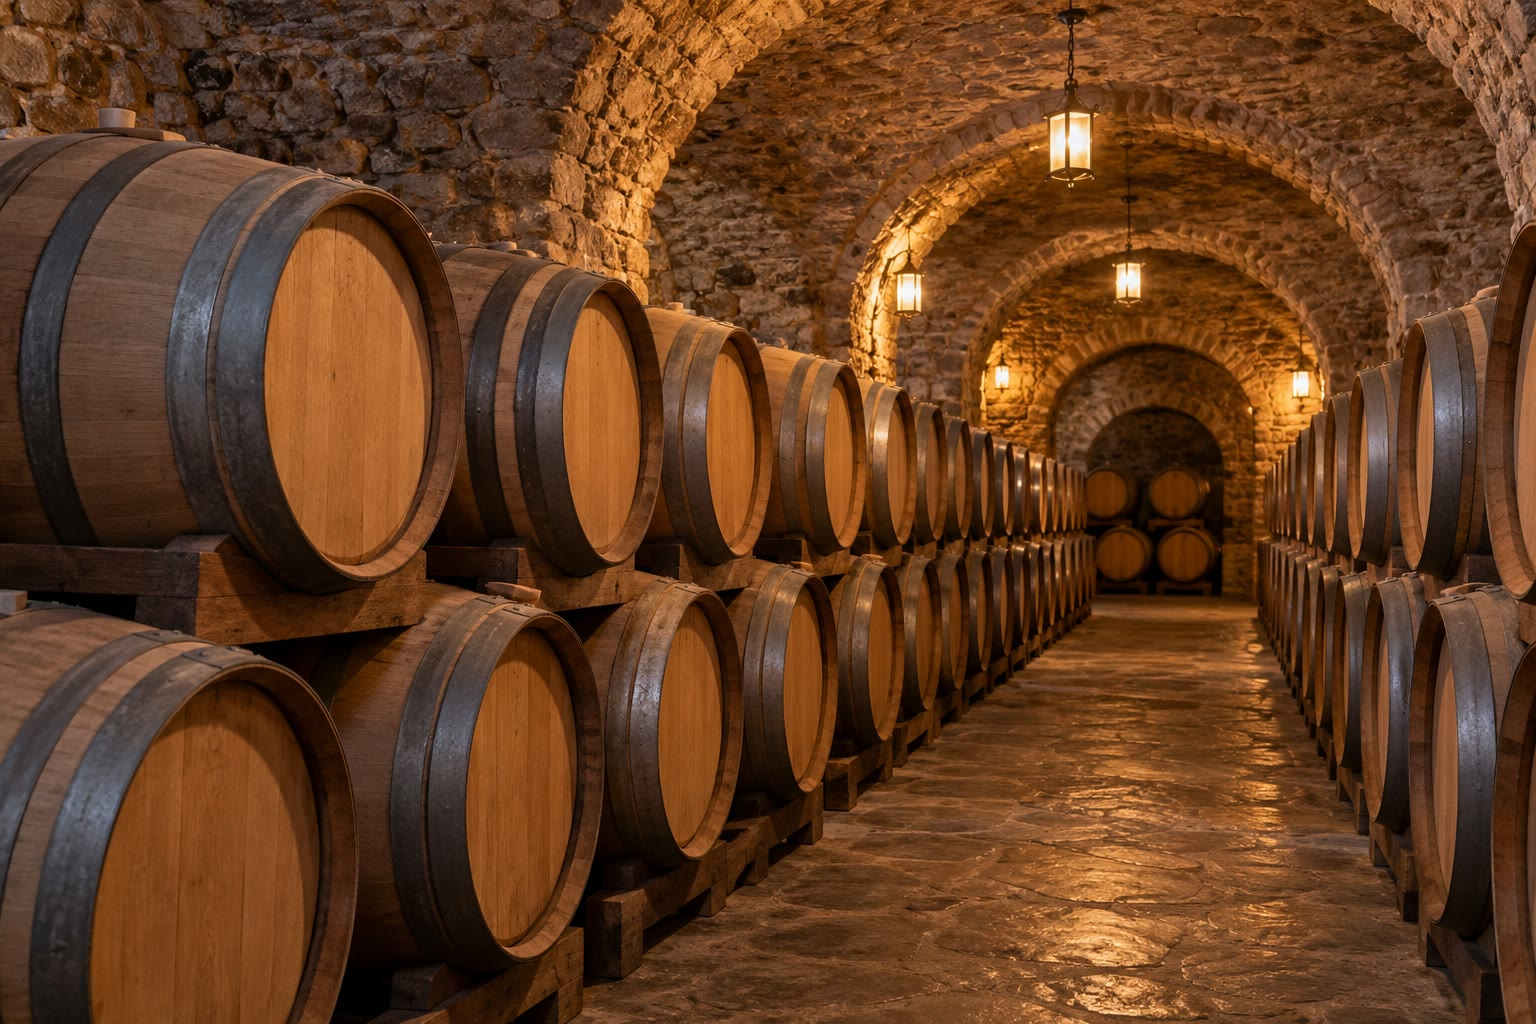
\includegraphics[width=0.58\linewidth]{images/book2/ai/b1-24-wine-cellar.jpg}

{\small نبيذ يتعتّق في قبو. فإذا حُفظ من الهواء، احتفظ النبيذ بإيثانوله؛
وإذا تعرّض للهواء، أكسدته بكتيريا حمض الخل إلى حمض الإيثانويك.}
\end{omfigure}

\section{مستويات أكسدة الكربون}

\begin{definition}[مستوى الأكسدة]\label{def:b1:organic-redox:oxidation-level}
\emph{مستوى الأكسدة}\index{مستوى الأكسدة} لذرة كربون هو
عدد أكسدتها، الذي يُحصل عليه بقواعد
\cref{prop:b1:nernst:on-rules}: كل رابطة مع ذرة أكثر كهرسلبية
(O، N، هالوجين) تُعدّ $+1$، وكل رابطة مع الهيدروجين $-1$، وكل رابطة مع
كربون آخر 0 (والرابطة الثنائية تُعدّ مرتين).
\end{definition}

\begin{proposition}[أعداد أكسدة الكربون]\label{prop:b1:organic-redox:on-of-carbon}
\omterm{def:b1:nernst:oxidation-number}{عدد أكسدة} الكربون يساوي (عدد الروابط مع O أو N أو
الهالوجينات) مطروحًا منه (عدد الروابط مع H). وضمن عائلة واحدة من المركبات
ذات الهيكل الكربوني نفسه، تكون السلسلة \babelsublr{\foreignlanguage{arabic}{كحول} $\to$ \foreignlanguage{arabic}{ألدهيد أو كيتون} $\to$
\foreignlanguage{arabic}{حمض كربوكسيلي} $\to$ \foreignlanguage{arabic}{ثنائي أكسيد الكربون}} سلسلة أكسدات يتبادل كل منها
إلكترونين.
\end{proposition}

\begin{proof}
بكسر كل رابطة وإعطاء الإلكترونين كليهما للشريك الأكثر
كهرسلبية: من H (الأقل كهرسلبية من C) يكسب الكربون إلكترونًا،
فالشحنة $-1$ لكل رابطة C--H؛ ومع O وN والهالوجينات (الأكثر كهرسلبية) يفقد
إلكترونًا، $+1$ لكل رابطة؛ وتُقسم الروابط C--C بالتساوي. وبالانتقال من \ce{-CH2OH}
($-1$ لكربون مرتبط بكربون آخر واحد) إلى \ce{-CHO} ($+1$) إلى
\ce{-COOH} ($+3$)، يرتفع العدد بمقدار 2 في كل خطوة: إلكترونان.
\end{proof}

\begin{omfigure}
\begin{tikzpicture}[font=\small, >={Stealth}]
  \foreach \x/\f/\n in {0/\ce{CH4}/-4, 2.4/\ce{CH3OH}/-2, 4.8/\ce{HCHO}/0, 7.2/\ce{HCOOH}/+2, 9.6/\ce{CO2}/+4} {
    \node[draw, rounded corners, minimum width=1.5cm] at (\x,0) {\f};
    \node[below] at (\x,-0.5) {$\n$};
  }
  \foreach \x in {0.8,3.2,5.6,8.0} \draw[->, thick, omThm] (\x,0) -- ++(0.8,0);
  \node[omThm, above] at (4.8,0.5) {\foreignlanguage{arabic}{أكسدة: $-2\,\mathrm{e^-}$ و$-2\,\ce{H+}$ في كل خطوة}};
  \node[left] at (-0.9,-0.75) {\foreignlanguage{arabic}{عدد أكسدة \babelsublr{C}:}};
\end{tikzpicture}

{\small \omterm{def:b1:organic-redox:oxidation-level}{مستويات أكسدة} عائلة الكربون الواحد: الميثان، والميثانول،
والميثانال، وحمض الميثانويك، وثنائي أكسيد الكربون. كل سهم أكسدة
بإلكترونين؛ وإذا قُرئ معكوسًا، فهو اختزال.}
\end{omfigure}

\begin{method}[موازنة نصف معادلة عضوية]\label{met:b1:organic-redox:balance-organic-redox}
\begin{enumerate}
  \item اكتب \omterm{def:b1:nernst:couple}{المؤكسد} \omterm{def:b1:nernst:couple}{والمختزل} العضويين بالهيكل نفسه.
  \item عُدّ الإلكترونات من تغيّر \omterm{def:b1:nernst:oxidation-number}{أعداد أكسدة}
        الكربونات التي تتغير (أو ببساطة: إلكترونان لكل زوج من H يُفقد، أو لكل O
        يُكتسب).
  \item وازن الأكسجين بالماء، والهيدروجين بالأيون \ce{H+}، والشحنة
        بالإلكترونات.
\end{enumerate}
من الإيثانول إلى حمض الإيثانويك: \ce{CH3CH2OH + H2O -> CH3COOH + 4H+ + 4e-}.
ومع ثنائي الكرومات المحمَّض (\ce{Cr2O7^2- + 14H+ + 6e- -> 2Cr^3+ + 7H2O})،
ثلاثة جزيئات إيثانول لكل أيوني ثنائي كرومات:
\ce{3CH3CH2OH + 2Cr2O7^2- + 16H+ -> 3CH3COOH + 4Cr^3+ + 11H2O}.
\end{method}

\section{أكسدة الكحولات}

\begin{proposition}[ما تعطيه الكحولات عند أكسدتها]\label{prop:b1:organic-redox:alcohol-oxidation}
يتأكسد الكحول الأولي \ce{RCH2OH} إلى الألدهيد \ce{RCHO}، ثم
(في الماء، مع \omterm{def:b1:nernst:couple}{مؤكسد} قوي) إلى الحمض الكربوكسيلي \ce{RCOOH}؛
والكحول الثانوي \ce{R2CHOH} إلى الكيتون \ce{R2CO}، الذي يقاوم
مزيدًا من الأكسدة؛ أما الكحول الثالثي \ce{R3COH} فلا يتأكسد دون
كسر رابطة C--C.
\end{proposition}

\begin{proof}
تنزع أكسدة الكحول هيدروجين OH وهيدروجينًا
من الكربون الحامل لمجموعة OH، فتتكوّن C=O. والكربون الحامل لمجموعة OH في الكحول الثالثي لا يحمل
مثل هذا الهيدروجين. والألدهيد ما زال يحمل H على كربون الكربونيل؛ وفي
الماء يتميأ جزئيًا، \ce{RCH(OH)2}، فيتأكسد من جديد بالطريقة
نفسها إلى \ce{RCOOH}. أما الكيتون فلا H على ذلك الكربون فيتوقف.
\end{proof}

المؤكسدات القوية في الماء --- ثنائي كرومات البوتاسيوم المحمَّض أو
البرمنغنات --- تؤكسد الكحولات الأولية إلى أحماض. وللتوقف عند
الألدهيد، يُقطَّر إلى الخارج كلما تكوّن (فالألدهيدات تغلي عند درجة أدنى من
الكحولات التي تأتي منها، لخلوها من \omterm{def:b1:intermolecular-forces-solvents:hbond}{الروابط الهيدروجينية} O--H)، أو تُستعمل كواشف
أخف لامائية، يصفها مجلد السنة الثانية.

\begin{safety}{\ghs[5mm]{GHS03}\,\ghs[5mm]{GHS05}\,\ghs[5mm]{GHS06}\,\ghs[5mm]{GHS07}\,\ghs[5mm]{GHS08}\,\ghs[5mm]{GHS09}}
ثنائي كرومات البوتاسيوم، \omterm{def:b1:nernst:couple}{المؤكسد} البرتقالي الكلاسيكي للكحولات،
مصنَّف ضمن المواد التي قد تسبب السرطان: فلا يُتداول إلا
بكميات صغيرة، مع القفازات والنظارات الواقية، وتُجمع فضلاته الكرومية
منفصلة؛ ويُفضَّل حيثما أمكن \omterm{def:b1:nernst:couple}{مؤكسد} أقل
خطرًا.
% ledger: ghs:K2Cr2O7
\end{safety}

\section{اختزال مركبات الكربونيل بالهيدريدات}

\begin{definition}[مانح الهيدريد]\label{def:b1:organic-redox:hydride-donor}
\emph{مانح الهيدريد}\index{مانح الهيدريد} ينقل ذرة هيدروجين مع
زوجها الرابط، \ce{H-}، إلى كربون \omterm{def:b1:electronic-effects:nucleophile}{محب للإلكترونات}. وبوروهيدريد الصوديوم
\ce{NaBH4} وهيدريد الليثيوم والألومنيوم \ce{LiAlH4} \emph{هيدريدات فلزية
معقدة}\index{هيدريد فلزي معقد}: إذ يُقدَّم الهيدريد
من الأيون \ce{BH4-} أو \ce{AlH4-}، لا على هيئة أيون حر.
\end{definition}

\begin{omfigure}
\setchemfig{atom sep=2.1em}
\schemestart
\chemfig{H_3B^{-}-[@{bh}]@{h}H}
\+
\chemfig{@{c}C(-[:150]R)(-[:210]R')=[@{co}]@{o}O}
\arrow{->}
\chemfig{C(-[:150]R)(-[:210]R')(-[2]H)-O^{-}}
\arrow{->[\ce{H2O}]}
\chemfig{C(-[:150]R)(-[:210]R')(-[2]H)-OH}
\schemestop
\chemmove{\draw[->, thick, shorten <=2pt, shorten >=3pt](bh) .. controls +(80:9mm) and +(180:7mm) .. (c);
          \draw[->, thick, shorten <=2pt, shorten >=2pt](co) .. controls +(90:6mm) and +(90:6mm) .. (o);}
\par\vspace{6pt}

{\small اختزال كيتون بالبوروهيدريد: يكوّن زوج B--H الرابطة C--H
الجديدة بينما يذهب زوج $\pi$ للرابطة C=O إلى الأكسجين؛ ويبرتن
المذيبُ (الماء أو الكحول) الألكوكسيدَ أو يُبرتَن عند المعالجة. ويستطيع كل \ce{BH4-}
أن يقدّم هيدروجيناته الأربعة تباعًا.}
\end{omfigure}

\begin{proposition}[مجال الهيدريدين]\label{prop:b1:organic-redox:hydride-scope}
بوروهيدريد الصوديوم، المستعمل في الماء أو الكحولات، يختزل الألدهيدات إلى
كحولات أولية والكيتونات إلى كحولات ثانوية، ويترك الإسترات،
والأحماض الكربوكسيلية، والأميدات والروابط الثنائية C=C دون مساس. أما هيدريد الليثيوم
والألومنيوم، المستعمل في إيثر جاف، فيختزل أيضًا الإسترات والأحماض
الكربوكسيلية إلى كحولات أولية، ويتفاعل بعنف مع الماء.
\end{proposition}

\begin{proof}
الرابطة Al--H أشد استقطابًا من الرابطة B--H (فالألومنيوم أقل
كهرسلبية من البور)، فيكون \ce{AlH4-} \omterm{def:b1:organic-redox:hydride-donor}{مانح هيدريد} أقوى بكثير،
قادرًا على مهاجمة الكربونيل الأقل محبةً للإلكترونات في الإسترات
والكربوكسيلات؛ والتفاعلية نفسها تجعله يتفاعل مع أي هيدروجين
حمضي، ومنه الماء. أما \ce{BH4-} فلا يتفاعل إلا ببطء مع الماء
والكحولات، ولا يهاجم إلا أشد مجموعات الكربونيل محبةً للإلكترونات. والرابطة
C=C المعزولة ليست محبة للإلكترونات ولا يختزلها أي منهما.
\end{proof}

\section{الانتقائية}

\begin{definition}[التفاعل الانتقائي كيميائيًا]\label{def:b1:organic-redox:chemoselective}
\emph{التفاعل الانتقائي كيميائيًا}\index{تفاعل انتقائي كيميائيًا} يؤثر في
مجموعة وظيفية واحدة من جزيء بوجود مجموعات أخرى كان يمكنها،
مع كاشف آخر، أن تتفاعل هي أيضًا.
\end{definition}

\begin{omfigure}
\begin{tabular}{lcc}
\hline
المجموعة & \ce{NaBH4} (مذيب كحولي) & \ce{LiAlH4} (إيثر جاف) \\
\hline
ألدهيد \ce{RCHO} & كحول أولي & كحول أولي \\
كيتون \ce{R2CO} & كحول ثانوي & كحول ثانوي \\
إستر \ce{RCOOR} & لا تفاعل & كحولان \\
حمض كربوكسيلي \ce{RCOOH} & لا تفاعل (ملح) & كحول أولي \\
ألكين \ce{C=C} & لا تفاعل & لا تفاعل \\
\omterm{def:b1:acetals-protection:hemiacetal}{أسيتال} & لا تفاعل & لا تفاعل \\
\hline
\end{tabular}

\smallskip
{\small ما يختزله الهيدريدان. بوروهيدريد الصوديوم هو
الكاشف الانتقائي كيميائيًا؛ وهيدريد الليثيوم والألومنيوم هو الكاشف القوي.}
\end{omfigure}

\begin{example}[إستر كيتوني]\label{ex:b1:organic-redox:ketoester}
يعطي 4-أوكسو بنتانوات الإيثيل، \ce{CH3CO(CH2)2COOEt}، مع بوروهيدريد الصوديوم
4-هيدروكسي بنتانوات الإيثيل: فلا يُختزل إلا الكيتون. ومع هيدريد الليثيوم
والألومنيوم، تُختزل المجموعتان كلتاهما: بنتان-1,4-ثنائي أول (و
الإيثانول). ولاختزال الإستر وحده، يجب أولًا \omterm{def:b1:acetals-protection:protecting-group}{حماية} الكيتون على هيئة
\omterm{def:b1:acetals-protection:hemiacetal}{أسيتال} (\cref{ch:b1:acetals-protection}).
\end{example}

\begin{inthelab}[اختزال كيتون]
يُضاف بوروهيدريد الصوديوم على دفعات صغيرة إلى محلول بارد من
الكيتون في الإيثانول: فالتفاعل ناشر للحرارة، ويفور الهيدروجين من
التفاعل البطيء للكاشف مع المذيب. وبعد التحريك، يهدم حمض
مخفف الفائض من الكاشف (مزيد من الهيدروجين: فلا لهب بالقرب) ثم
يُستخلص الكحول. أما هيدريد الليثيوم والألومنيوم فلا يُستعمل، على العكس من ذلك،
إلا في إيثر جاف تحت غاز خامل، ويُهدم فائضه بعناية
شديدة.
\end{inthelab}

\section{تمارين}

\begin{exercise}[$\star$]\label{exo:b1:organic-redox:1}
أعطِ \omterm{def:b1:nernst:oxidation-number}{عدد أكسدة} كل كربون في الإيثانول، والإيثانال، وحمض
الإيثانويك، والبروبانون وحمض الميثانويك.
\end{exercise}

\begin{exercise}[$\star$]\label{exo:b1:organic-redox:2}
ماذا يعطي ثنائي الكرومات المحمَّض مع البروبان-1-أول، والبروبان-2-أول
و2-ميثيل البروبان-2-أول؟
\end{exercise}

\begin{exercise}[$\star$]\label{exo:b1:organic-redox:3}
اكتب نصفي معادلتي المزدوجتين بروبانون/بروبان-2-أول
وإيثانال/إيثانول في الوسط الحمضي.
\end{exercise}

\begin{exercise}[$\star$]\label{exo:b1:organic-redox:4}
ماذا يعطي بوروهيدريد الصوديوم وهيدريد الليثيوم والألومنيوم مع
البوتانال، والبوتانون، وبوتانوات الإيثيل وحمض البوتانويك؟
\end{exercise}

\begin{exercise}[$\star\star$]\label{exo:b1:organic-redox:5}
وازن أكسدة البروبان-2-أول بالبرمنغنات في الوسط الحمضي
($\ce{MnO4-}/\ce{Mn^2+}$) واحسب حجم البرمنغنات ذات التركيز
\qty{0.020}{mol/L} اللازم لأكسدة \qty{1.20}{g} من الكحول ($M = \qty{60.0}{g/mol}$).
\end{exercise}

\begin{exercise}[$\star\star$]\label{exo:b1:organic-redox:6}
كيف يمكن الحصول على البروبانال من البروبان-1-أول دون أن يتأكسد
أكثر؟ استعمل درجتي الغليان: البروبان-1-أول \qty{97}{\celsius}، والبروبانال
\qty{48}{\celsius}.
% ledger: bp:propanal, bp:propan-1-ol
\end{exercise}

\begin{exercise}[$\star\star$]\label{exo:b1:organic-redox:7}
اكتب آلية اختزال الإيثانال بالأيون \ce{BH4-} في الإيثانول.
أي ذرة من الناتج تأتي من الكاشف؟
\end{exercise}

\begin{exercise}[$\star\star$]\label{exo:b1:organic-redox:8}
يعطي اختزال البوتان-2-ون بالكاشف \ce{NaBH4} كحولًا \omterm{def:b1:stereochemistry-in-depth:stereocentre}{كيراليًا}. هل هو
نشط ضوئيًا؟ ولماذا؟
\end{exercise}

\begin{exercise}[$\star\star$]\label{exo:b1:organic-redox:9}
في اختبار النَّفَس الكحولي الذي استعملته الشرطة قديمًا، كان ثنائي الكرومات البرتقالي
يتحول إلى الأخضر. اكتب التفاعل مع الإيثانول وفسّر تغيّر
اللون.
\end{exercise}

\begin{exercise}[$\star\star\star$]\label{exo:b1:organic-redox:10}
اقترح تخليقين: 2-ميثيل بوتان-2-أول من الإيثانال \omterm{def:b1:organomagnesium:organometallic}{وكاشف غرينيار}
تليهما أكسدة ثم خطوة غرينيار ثانية؛ والبنتان-3-أول
من البروبانال. وعُدّ عمليات الأكسدة والاختزال.
\end{exercise}

\begin{exercise}[$\star\star\star$]\label{exo:b1:organic-redox:11}
اختزل مجموعة الإستر وحدها في 4-أوكسو بنتانوات الميثيل،
\ce{CH3CO(CH2)2COOCH3}. خطّط للخطوات الثلاث مع \omterm{def:b1:acetals-protection:protecting-group}{حماية} وأعطِ
الناتج.
\end{exercise}

\begin{exercise}[$\star\star\star$]\label{exo:b1:organic-redox:12}
بيّن أن أكسدة كحول أولي إلى الحمض يُتبادل فيها أربعة
إلكترونات، \omterm{def:b1:nernst:oxidation-number}{بأعداد الأكسدة} وبنصف
المعادلة. وعمّم ذلك على أكسدة الميثان إلى ثنائي أكسيد الكربون.
\end{exercise}

\section{مسألة: من الهكسانول الحلقي إلى حمض الأديبيك}

\begin{problem}[{مسألة نهاية الأسبوع --- مستويات الأكسدة في الهكسانول الحلقي،
والهكسانون الحلقي وحمض الأديبيك، والأكسدة بحمض النتريك
وإلكتروناتها، وطريق بفوق أكسيد الهيدروجين، وكتلة أكسيد ثنائي النيتروجين
المنطلقة لكل طن من حمض الأديبيك}]
\label{pb:b1:organic-redox:1}
حمض الأديبيك، أي حمض الهكسان ثنائي الأويك \ce{HOOC(CH2)4COOH}، يُصنع على نطاق واسع
من أجل النيلونات، وغالبًا بأكسدة الهكسانول الحلقي (مع الهكسانون الحلقي)
بحمض النتريك، الذي يطلق أكسيد ثنائي النيتروجين \ce{N2O}، وهو غاز دفيئة
قوي. الكتل المولية (\unit{g/mol}): \ce{C6H12O} 100.0،
\ce{C6H10O} 98.0، \ce{C6H10O4} 146.0، \ce{N2O} 44.0، \ce{HNO3} 63.0،
\ce{H2O2} 34.0.

\medskip
\noindent\textbf{الجزء الأول --- \omterm{def:b1:organic-redox:oxidation-level}{مستويات الأكسدة}.}
\begin{enumerate}
  \item أعطِ \omterm{def:b1:nernst:oxidation-number}{عدد أكسدة} كل كربون في الهكسانول الحلقي.
  \item والسؤال نفسه للهكسانون الحلقي.
  \item والسؤال نفسه لحمض الأديبيك.
  \item أي الكربونات تتأكسد في الانتقال من الهكسانول الحلقي إلى حمض
        الأديبيك، وأي رابطة تنكسر؟
  \item كم إلكترونًا يفقد جزيء واحد من الهكسانول الحلقي؟
  \item لماذا يتأكسد الهكسانون الحلقي، وهو كيتون، أكثر هنا مع ذلك؟
\end{enumerate}

\medskip
\noindent\textbf{الجزء الثاني --- طريق حمض النتريك.}
\begin{enumerate}[resume]
  \item اكتب \omterm{def:b1:nernst:couple}{نصف معادلة} تحول الهكسانول الحلقي إلى حمض الأديبيك في الوسط الحمضي.
  \item أعطِ \omterm{def:b1:nernst:oxidation-number}{عدد أكسدة} N في \ce{HNO3} وفي \ce{N2O}.
  \item اكتب \omterm{def:b1:nernst:couple}{نصف المعادلة} $\ce{HNO3}/\ce{N2O}$.
  \item اجمعهما؛ وتحقق من أنك تحصل على
        \ce{C6H12O + 2HNO3 -> C6H10O4 + N2O + 2H2O}.
  \item كم مولًا من الإلكترونات يُتبادل لكل مول من حمض
        الأديبيك؟
  \item احسب كتلة حمض النتريك المستهلكة لكل طن من حمض الأديبيك.
\end{enumerate}

\medskip
\noindent\textbf{الجزء الثالث --- طريق بفوق أكسيد الهيدروجين.}
\begin{enumerate}[resume]
  \item اكتب \omterm{def:b1:nernst:couple}{نصف المعادلة} $\ce{H2O2}/\ce{H2O}$.
  \item اكتب أكسدة الهكسانول الحلقي بفوق أكسيد
        الهيدروجين إلى حمض الأديبيك ووازنها.
  \item احسب كتلة \ce{H2O2} لكل طن من حمض الأديبيك.
  \item ما الناتج الجانبي الوحيد؟ ولماذا يوصف هذا الطريق بأنه أكثر خضرة؟
  \item يجب تنشيط فوق أكسيد الهيدروجين \omterm{def:b1:elementary-steps:catalyst}{بحفّاز}. مستعينًا
        بما جاء في \cref{exo:b1:nernst:12}، فسّر لماذا قد تحتاج أكسدة محابية
        ديناميكيًا حراريًا إلى \omterm{def:b1:elementary-steps:catalyst}{حفّاز} مع ذلك.
  \item ماذا كان سيفعل بوروهيدريد الصوديوم بالهكسانون الحلقي؟ اكتب
        التفاعل.
\end{enumerate}

\medskip
\noindent\textbf{الجزء الرابع --- الكتل وغاز الدفيئة.}
\begin{enumerate}[resume]
  \item احسب كمية حمض الأديبيك في طن واحد.
  \item احسب كمية \ce{N2O} المتكوّنة معها بطريق حمض النتريك.
  \item احسب كتلة الهكسانول الحلقي اللازمة لكل طن، \omterm{def:b1:extent-q-and-k:fractional-extent}{بمردود}
        \qty{95}{\percent}.
  \item اذكر كتلة \ce{N2O} المنطلقة لكل طن من حمض الأديبيك بطريق
        حمض النتريك، بالأطنان.
\end{enumerate}
\end{problem}
